%%%%%%%%%%%%%%%%%%%%%%%%%%%%%%%%%%%%%%%%%%%%%%%%%%%%%%%%%%%%%%%%%%%%%%%%
% Plantilla TFG/TFM
% Escuela Politécnica Superior de la Universidad de Alicante
% Realizado por: Jose Manuel Requena Plens
% Contacto: info@jmrplens.com / Telegram:@jmrplens
%%%%%%%%%%%%%%%%%%%%%%%%%%%%%%%%%%%%%%%%%%%%%%%%%%%%%%%%%%%%%%%%%%%%%%%%

\chapter{Introduction}

Obesity represents a pressing global public health concern, affecting a
significant segment of the population. In a previous initiative, \todo{link}
Tech4Diet developed a system enabling patients undergoing weight loss treatment
to visualize 3D scans of their bodies throughout their weight loss
journey~\cite{Azorin-Lopez2020}.

During the treatment, the patient's body is captured using an RGBD camera, the
Intel RealSense D435. The 3D model of the human body is shown during the
different sessions using a virtual reality headset. This innovative approach
aimed to boost motivation and increase treatment plan adherence.

\begin{figure}
      \centering
      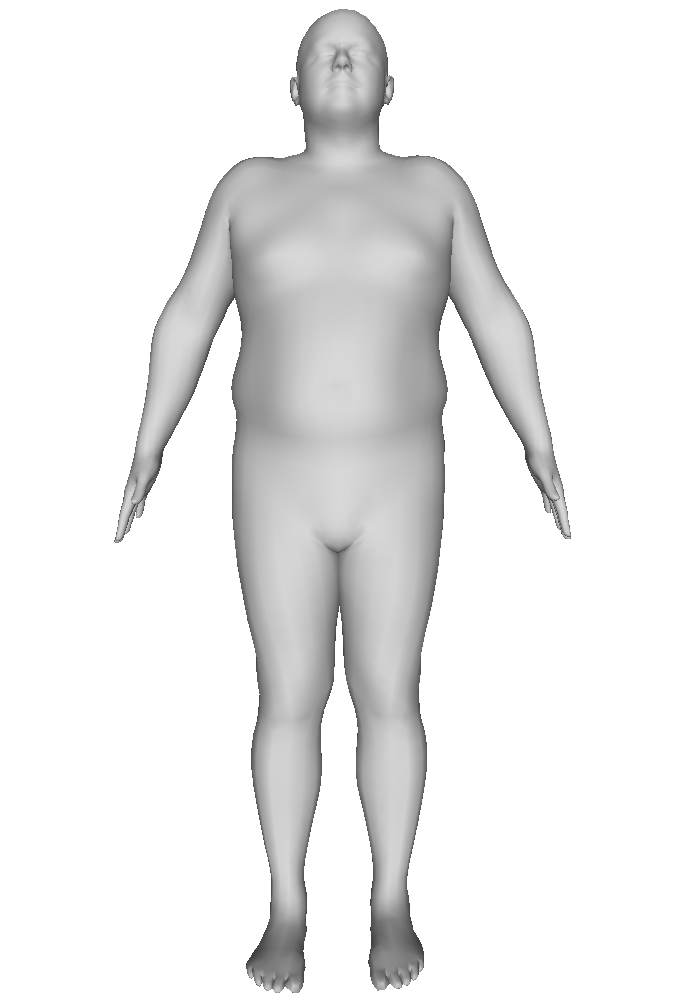
\includegraphics[width=75pt]{files/patient_8/2_cropped}
      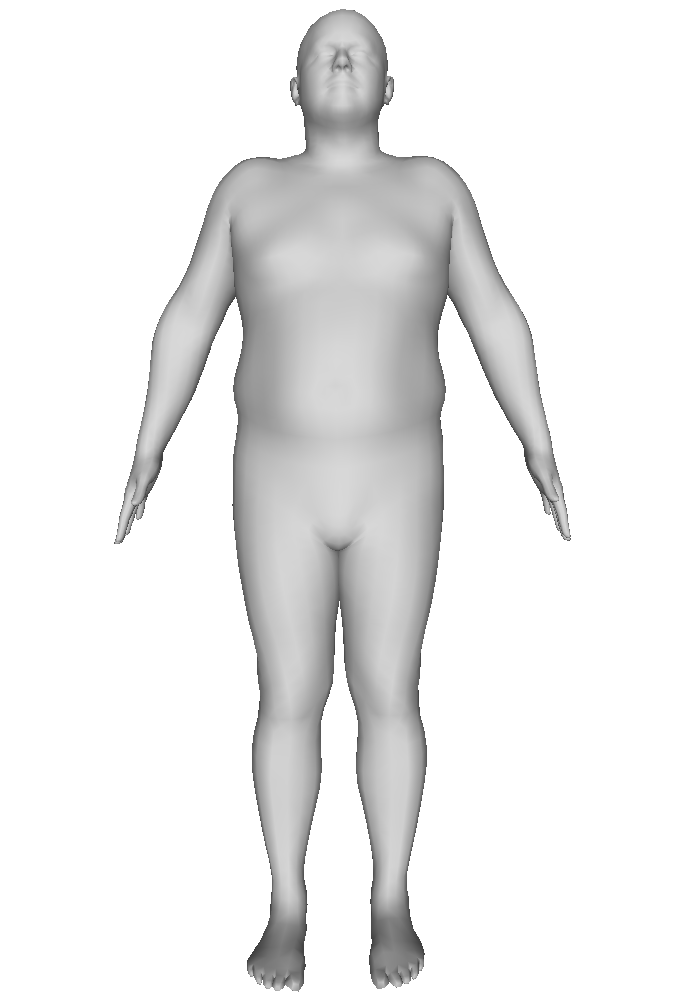
\includegraphics[width=75pt]{files/patient_8/3_cropped}
      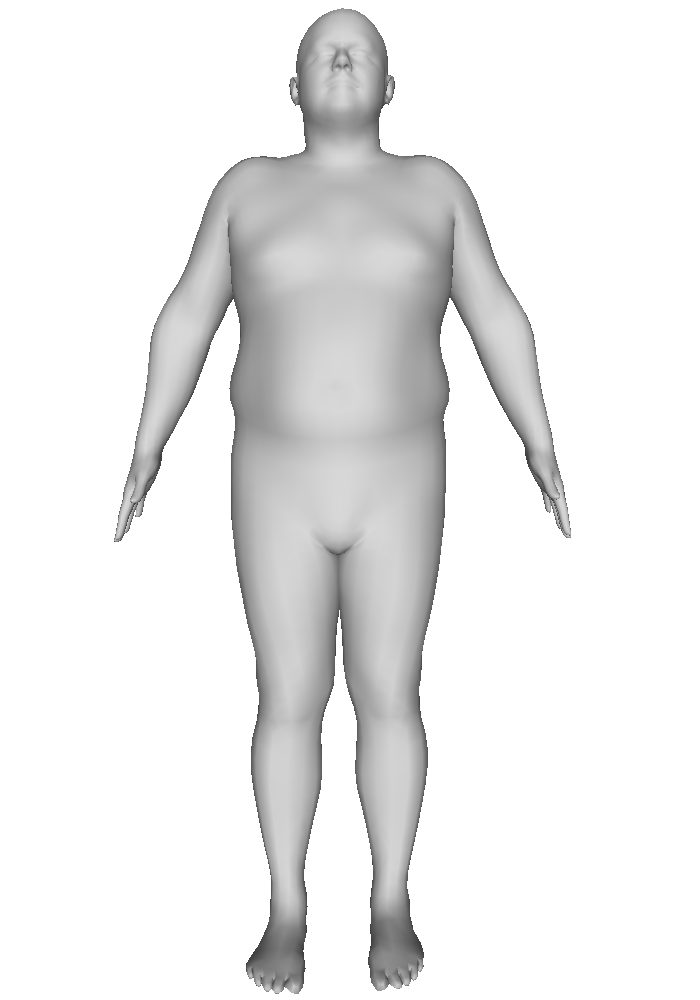
\includegraphics[width=75pt]{files/patient_8/4_cropped}
      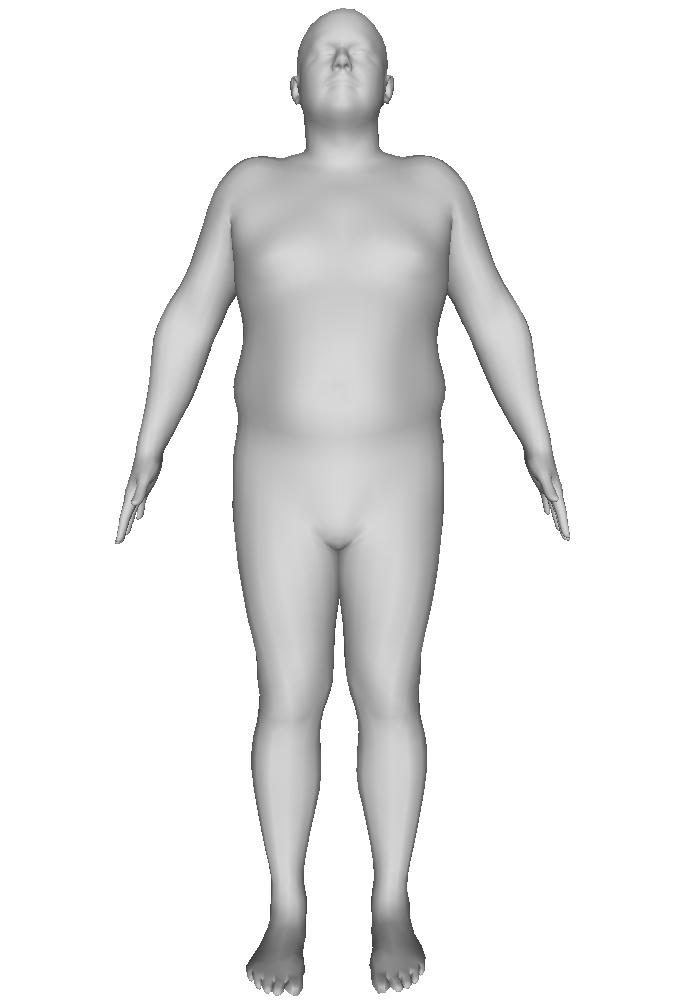
\includegraphics[width=75pt]{files/patient_8/5_cropped}
      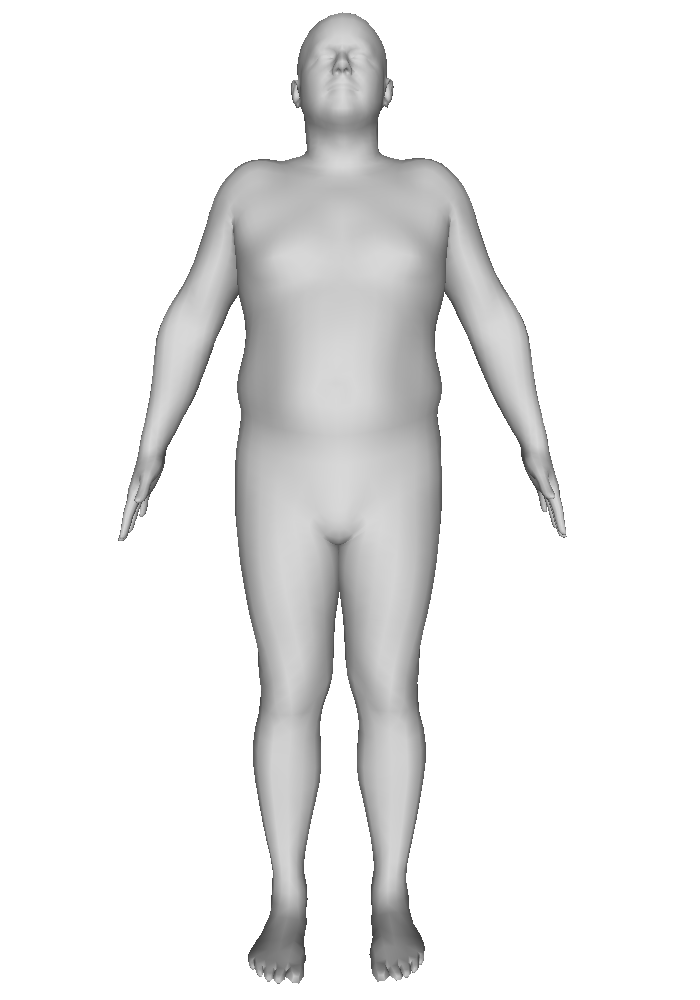
\includegraphics[width=75pt]{files/patient_8/6_cropped}
      \caption{3D model reconstruction of a patient's body at different stages of a weight loss
            treatment. There is around a month between each scan, and a total
            weight loss of 3.8 kg.}
\end{figure}

Subsequently, we wondered if it would be feasible to utilize the datasets
acquired in this prior study to formulate a predictive model. This model would
project anticipated changes in a person's body undergoing weight loss treatment
before the treatment concludes, further bolstering adherence to the treatment
regimen. The present work explores the development of such a model. This
includes analyzing data from the earlier study, reviewing existing techniques
in human body model representation, encoding patient data using the chosen
representation, devising a neural network architecture for predicting patient
body changes, and finally, training and evaluating the model.

\section{3D human body model applications}

There are many areas that can make use of these models. Some of the most
significant applications include:

\begin{itemize}
      \item Medicine: Human body models are valuable in the study of
            anatomy~\cite{https://doi.org/10.1002/ase.1718} and for patient monitoring.
      \item Film industry: Human body models can be used to capture motion data and render
            high-quality CGI humans.
      \item Video game industry: Human body models can be used to create realistic
            animations and interactions between characters\cite{Starke2021}.
      \item Extended reality: Human body models can be used to capture user input in
            virtual reality as well as rendering realistic characters.
      \item Clothing: These models can be used for fitting virtual
            clothes\cite{apeagyei2010application} and creating realistic images of clothing
            products.
\end{itemize}